
\section{High Availability}
\label{sec:availability}

To understand which guarantees can be provided with high availabilty,
we must first understand what properties define high availability. In
this section, we will formulate a model that captures a range of
availability models, including ``true'' high availability,
availablility with stickiness, and several other useful variants.

Informally, highly available algorithms ensure ``always on'' operation
and promise a guaranteed response. If users of a highly available
system are able to contact a (set of) server(s) in a system, they are
guaranteed a response as the (set of) server(s) does not need to
communicate with any others. This lack of fast-path coordination also
means that a highly available system can also offer low latency
operation~\cite{abadi-pacelc}. To describe whether a transactional
system is highly available, we need both a way to describe what
servers a client must contact as well as what kinds of responses a
server can provide, especially given the possibility of aborts.

\subsection{Replica Availability}

Traditionally, a system provides high availability if every user that
can contact a server eventually receives a response from that server,
even in the presence of arbitrary, indefinitely long network
partitions between servers~\cite{gilbert-cap}. This is a useful
definition: if we can contact at least one server, then we can receive
a response. However, there are several other cases we should consider.

First, clients may wish to contact multiple servers. For example, to
ensure that the effects of its operations will persist in the face of
server failures, clients may wish to wait until operations reach more
than one server before they considers operations completed. However,
according to our definition of high availability, server-fault
tolerance is unavailable. To allow flexibility in the number of
servers required for an operation, we propose
\textit{$K$-availability}: if a client can contact $K$ servers, then
it eventually receives a response from all of them, even in the
presence of indefinitely long network partitions. Compared to a system
providing high availability ($1$-availability), a system with
$2$-availability and will require more messaging, possibly higher
latency and more unsuccessful operations in the presence of network
and server failures.  Additionally, as is commmon in standard
consensus algorithms like Paxos, clients may want to contact a
majority of $N$ servers in a system. This \textit{majority
  availability} (a special case of $K$-availability with $K=\lceil
\frac{N}{2} \rceil$) is more available than $N$-availability.

Clients may also wish to contact the same server (or set of servers)
across subsequent operations. As we will discuss in
Section~\ref{sec:hats}, clients can ensure continuity between
operations (e.g., reading their prior updates to a data item) by
maintaining affinity or ``stickiness'' with a server or set of
servers~\cite{vogels-defs}. Simultaneously aintaining availability and
stickiness requires fate-sharing between the client and its set of
servers: if a client's sticky servers fail, or, equivalently, if the
client is partitioned from its sticky servers, then it may face
unavailability. We say that a system provides \textit{sticky
  availability} if a client's subsequent operations are executed
against a server that has observed all of its prior operations, then
it eventually receives a response, even in the presence of
indefinitely long partitions. As above, it may be useful for a client
to achieve stickiness \textit{and} contact many replicas (i.e., for
fault tolerance), so we generalize sticky availability to
\textit{$K$-sticky availability}, which provides sticky availability
with $K$ distinct servers. A client may choose to become $1$-sticky
available by acting as a server itself; for example, a client might
cache its reads and writes. However, a single client cannot achieve
$K$-sticky availability with $K>1$ on its own. Moreover, ``sticking''
all clients to a designated set of servers (i.e., master availability)
is a special case of sticky availability and is less available than
the equivalent sticky availability.

\begin{figure}
\centering
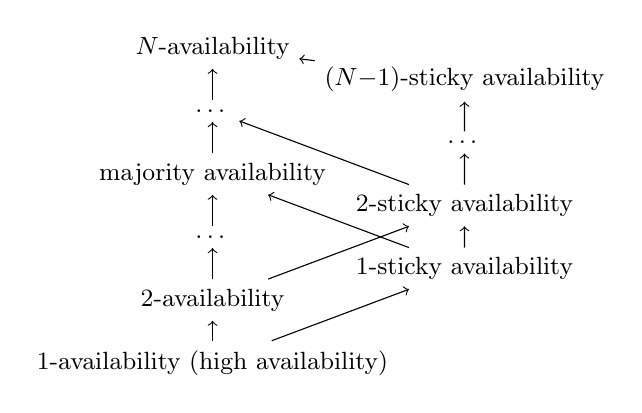
\begin{tikzpicture}[scale=0.8]
  \tikzstyle{every node}=[font=\small]
 \node[draw=none,fill=none] (1) at (0,0) {$1$-availability (high availability)}; 
 \node[draw=none,fill=none] (2) at (0,1) {$2$-availability}; 
 \node[draw=none,fill=none] (m-1) at (0, 2) {\ldots}; 
 \node[draw=none,fill=none] (m) at (0, 3) {majority availability}; 
 \node[draw=none,fill=none] (m+1) at (0, 4) {\ldots}; 
 \node[draw=none,fill=none] (n) at (0, 5) {$N$-availability}; 
 \node[draw=none,fill=none] (1s) at (4, 1.5) {$1$-sticky availability};
 \node[draw=none,fill=none] (2s) at (4, 2.5) {$2$-sticky availability};
 \node[draw=none,fill=none] (n2s) at (4, 3.5) {\ldots};
 \node[draw=none,fill=none] (n1s) at (4, 4.5) {$(N$$-$$1)$-sticky availability};

 \draw [->] (1) -- (2);
 \draw [->] (2) -- (m-1);
 \draw [->] (m-1) -- (m);
 \draw [->] (m) -- (m+1);
 \draw [->] (m+1) -- (n);
 \draw [->] (1) -- (1s);
 \draw [->] (1s) -- (m);
 \draw [->] (2s) -- (m+1);
 \draw [->] (1s) -- (2s);
 \draw [->] (2) -- (2s);
 \draw [->] (2s) -- (n2s);
 \draw [->] (n2s) -- (n1s);
 \draw [->] (n1s) -- (n);


\end{tikzpicture}
\label{fig:availability-order}
\caption{Hierarchy of replica availability levels for $N>3$ servers.}
\end{figure}

We show the hierarchy of replica availabilty levels in
Figure~\ref{fig:availability-order}. $K$-sticky availability subsumes
$K$-availability, but $K$-sticky availability is incomparable with
$(K+1)$-availability. $N$-sticky availability is equivalent to
$N$-availability, while majority availability subsumes $1$-sticky
availability More generally, $\lceil \frac{N}{2} \rceil$$+$$K$$-$$1$
availability subsumes $K$-sticky availability. We have omitted
discussion of operation-specific availability levels (e.g.,
$N$-availability for writes and $1$-availability for reads in a
write-all, read-one data store), system membership changes, or
heterogeneous replicas (e.g., servers in a local and remote
datacenters) but believe there are several avenues for further
taxnomization.

\subsection{Transactional Availability}

Thus far, we have focused on single-operation availability. This is
standard in distributed systems literature (e.g., atomic, regular, and
safe register models all concern single objects~\cite{herlihy-art}),
yet the database literature largely focuses on transactions: groups of
multiple operations over multiple objects. Accordingly, by itself,
replica availability is insufficient to describe availability
guarantees for transactions. Additionally, given the choice of
\textit{commit} and \textit{abort} responses---which signal
transaction success or failure to a client---we must be careful in
defining availability.

If a client wishes to execute a transaction that performs operations
on multiple data items, then the client must be able to contact and
receive a response from at least one server responsible for each data
item. This may result in lower availability than a non-transactional
requirement. Additionally, given the possiblity of aborts, we need to
ensure useful forward progress. A system can trivially guarantee
clients a response by always aborting their
transactions~\cite{transaction-liveness}. However, this is an
unsatisfactory system because nothing good (transaction commit) ever
happens; instead, we require a \textit{liveness} property. We cannot
guarantee that every transaction will commit---transactions may choose
to abort themselves---but we need to make sure that the system will
not indefinitely abort transactions on its own volition. We call a
transaction abort due to a transaction's own choosing (e.g., as part
of the transaction itself or due to a would-be integrity constraint
violation) an \textit{internal abort} and an abort due to system
implementation an \textit{external abort}.

We say that a system provides \textit{transactional availability} if,
given replica availability for every data item in a transaction, the
transaction eventually commits or internally aborts. For example,
system will violate transactional $2$-availability if client that can
contact two servers for each of data items in its transaction does not
eventually commit in the absence of internal aborts.

